\documentclass[12pt]{extarticle}

\usepackage{amsmath}
\usepackage{amsfonts}
\usepackage{graphicx}
\usepackage{nicefrac}
\usepackage{subfigure}
\usepackage{algorithm}
\usepackage{paralist}
\usepackage[geometry]{ifsym}
\usepackage{rotating}
\usepackage[normalem]{ulem}
\usepackage{varwidth}
% \usepackage{cite}
% \usepackage{color}
\usepackage{algpseudocode}
% \bibliographystyle{amsplain}




\usepackage[utf8]{inputenc}

% Default fixed font does not support bold face
\DeclareFixedFont{\ttb}{T1}{txtt}{bx}{n}{12} % for bold
\DeclareFixedFont{\ttm}{T1}{txtt}{m}{n}{12}  % for normal

% Custom colors
\usepackage{color}
\definecolor{deepblue}{rgb}{0,0,0.5}
\definecolor{deepred}{rgb}{0.6,0,0}
\definecolor{deepgreen}{rgb}{0,0.5,0}

\usepackage{listings}

% Python style for highlighting
\newcommand\pythonstyle{\lstset{
language=Python,
basicstyle=\ttm,
otherkeywords={self},             % Add keywords here
keywordstyle=\ttb\color{deepblue},
emph={MyClass,__init__},          % Custom highlighting
emphstyle=\ttb\color{deepred},    % Custom highlighting style
stringstyle=\color{deepgreen},
frame=tb,                         % Any extra options here
showstringspaces=false            %
}}


% Python environment
\lstnewenvironment{python}[1][]
{
\pythonstyle
\lstset{#1}
}
{}

% Python for external files
\newcommand\pythonexternal[1]{{
\pythonstyle
\lstinputlisting{#1}}}

% Python for inline
\newcommand\pythoninline[1]{{\pythonstyle\lstinline!#1!}}


\addtolength{\oddsidemargin}{-.2in}
    \addtolength{\evensidemargin}{-.5in}
    \addtolength{\textwidth}{0.5in}

    \addtolength{\topmargin}{-.5in}
    \addtolength{\textheight}{0.35in}

\sloppy                 % makes TeX less fussy about line breaking

\pagestyle{plain}           % use just a plain page number

\numberwithin{equation}{section}    % add the section number to the equation label

\usepackage{fancyheadings}

\newcommand{\com}[1]{\texttt{#1}}
\newcommand{\DIV}{\ensuremath{\mathop{\mathbf{DIV}}}}
\newcommand{\GRAD}{\ensuremath{\mathop{\mathbf{GRAD}}}}
\newcommand{\CURL}{\ensuremath{\mathop{\mathbf{CURL}}}}
\newcommand{\CURLt}{\ensuremath{\mathop{\overline{\mathbf{CURL}}}}}
\newcommand{\nullspace}{\ensuremath{\mathop{\mathrm{null}}}}


\newcommand{\FrameboxA}[2][]{#2}
\newcommand{\Framebox}[1][]{\FrameboxA}
\newcommand{\Fbox}[1]{#1}

%\usepackage[round]{natbib}

\newcommand{\half}{\mbox{\small \(\frac{1}{2}\)}}
\newcommand{\hf}{{\frac 12}}
\newcommand {\HH}  { {\bf H} }
\newcommand{\hH}{\widehat{H}}
\newcommand{\hL}{\widehat{L}}
\newcommand{\bmath}[1]{\mbox{\bf #1}}
\newcommand{\hhat}[1]{\stackrel{\scriptstyle \wedge}{#1}}
\newcommand{\R}{{\rm I\!R}}
\newcommand {\D} {{\vec{D}}}
\newcommand {\sg}{{\hsigma}}
%\renewcommand{\vec}[1]{\ensuremath{\mathbf{#1}}}
\newcommand{\E}{\vec{E}}
\renewcommand{\H}{\vec{H}}
\newcommand{\J}{\vec{J}}
\newcommand{\dd}{d^{\rm obs}}
% \newcommand{\F}{\vec{F}}
\newcommand{\C}{\vec{C}}
\newcommand{\s}{\vec{s}}
\newcommand{\N}{\vec{N}}
\newcommand{\M}{\vec{M}}
\newcommand{\A}{\vec{A}}
\newcommand{\B}{\vec{B}}
\newcommand{\w}{\vec{w}}
\newcommand{\nn}{\vec{n}}
\newcommand{\cA}{{\cal A}}
\newcommand{\cQ}{{\cal Q}}
\newcommand{\cR}{{\cal R}}
\newcommand{\cG}{{\cal G}}
\newcommand{\cW}{{\cal W}}
\newcommand{\hsig}{\hat \sigma}
\newcommand{\hJ}{\hat \J}
\newcommand{\hbeta}{\widehat \beta}
\newcommand{\lam}{\lambda}
\newcommand{\dt}{\delta t}
\newcommand{\kp}{\kappa}
\newcommand {\lag} { {\cal L}}
\newcommand{\zero}{\vec{0}}
\newcommand{\Hr}{H_{red}}
\newcommand{\Mr}{M_{red}}
\newcommand{\mr}{m_{ref}}
\newcommand{\thet}{\ensuremath{\mbox{\boldmath $\theta$}}}
\newcommand{\curl}{\ensuremath{\nabla_{\wedge}\,}}
\renewcommand{\div}{\nabla\cdot\,}
\newcommand{\grad}{\ensuremath{\nabla}}
\newcommand{\dm}{\delta m}
\newcommand{\gradh}{\ensuremath{\nabla}_h}
\newcommand{\divh}{\nabla_h\cdot\,}
\newcommand{\curlh}{\ensuremath{\nabla_h\times\,}}
\newcommand{\curlht}{\ensuremath{\nabla_h^T\times\,}}
\newcommand{\Q}{\vec{Q}}
\renewcommand{\J}{\vec J}
\renewcommand{\J}{\vec J}
\renewcommand{\u}{\vec u}
\newcommand{\f}{\vec f}
\newcommand{\n}{\vec n}
\renewcommand{\v}{\vec v}
\newcommand{\phiv}{\vec \phi}
% \usepackage[authoryear,numbers,square,sort,comma,colon,]{natbib}
% \usepackage[numbers/]{natbib}
% \usepackage[square,sort,comma,numbers]{natbib}
\renewcommand{\ne}{N\'ed\'elec elements }


\newcommand{\me}{Maxwell's equations }

\newcommand{\partialt}[1]{\frac{\partial #1}{\partial t}}
\newcommand{\cref}[1]{(\ref{#1})}
% \newcommand{\Ct}{\ensuremath{C^{\mbox{\tiny{T}}}}
\newcommand{\Ct}{\ensuremath{C^{\mbox{\tiny{T}}}}}
% \renewcommand{\baselinestretch}{1.40}\normalsize
\usepackage{setspace}
\usepackage{amsthm}
\newtheorem{prop}{Proposition}[section]
\DeclareMathAlphabet{\mathpzc}{OT1}{pzc}{m}{it}

\DeclareFontFamily{OT1}{pzc}{}
\DeclareFontShape{OT1}{pzc}{m}{it}{<-> s * [0.900] pzcmi7t}{}
\DeclareMathAlphabet{\mathpzc}{OT1}{pzc}{m}{it}

\onehalfspacing
\begin{document}
\pagestyle{fancyplain}
\fancyhead{}
\fancyfoot{} % clear all footer fields
\fancyfoot[LE,RO]{\thepage \hspace{-5mm}}
\fancyfoot[LO,CE]{ \footnotesize{ Michael Wathen 7830121}}
\fancyfoot[CO,RE]{}
% \pagecolor{cyan}










\section*{DG scalar Laplacian}

\begin{figure}[h!]
\centering
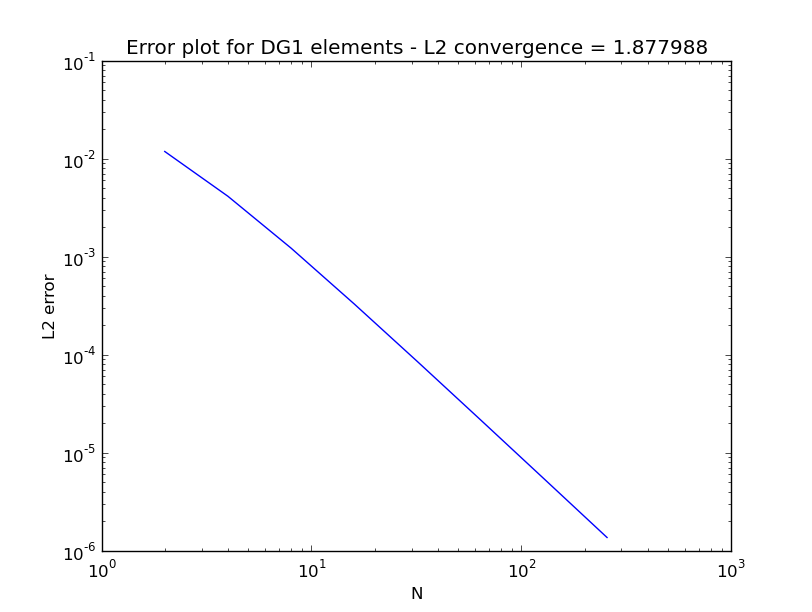
\includegraphics[width=10cm]{Plots/DGlapL2}
\end{figure}

\begin{figure}[h!]
\centering
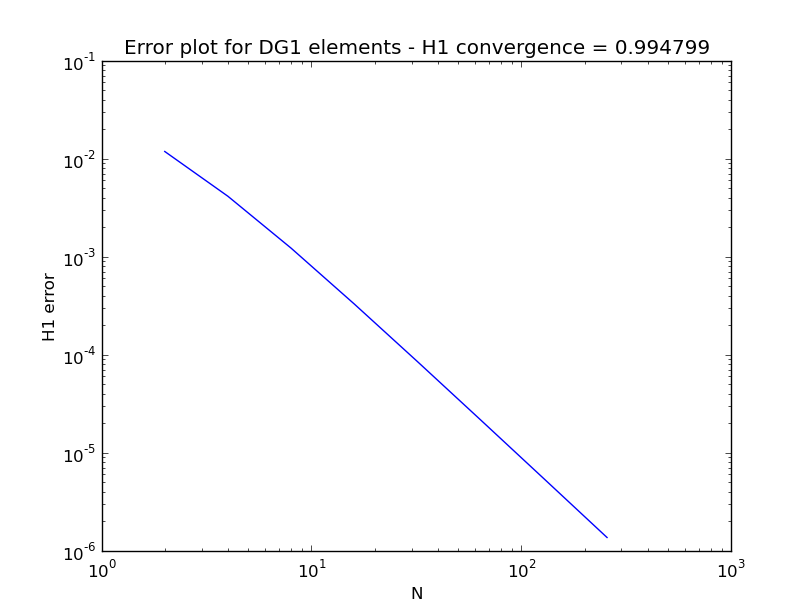
\includegraphics[width=10cm]{Plots/DGlapH1}
\end{figure}

top
\section*{BDM vector Laplacian}

\begin{figure}[h!]
\centering
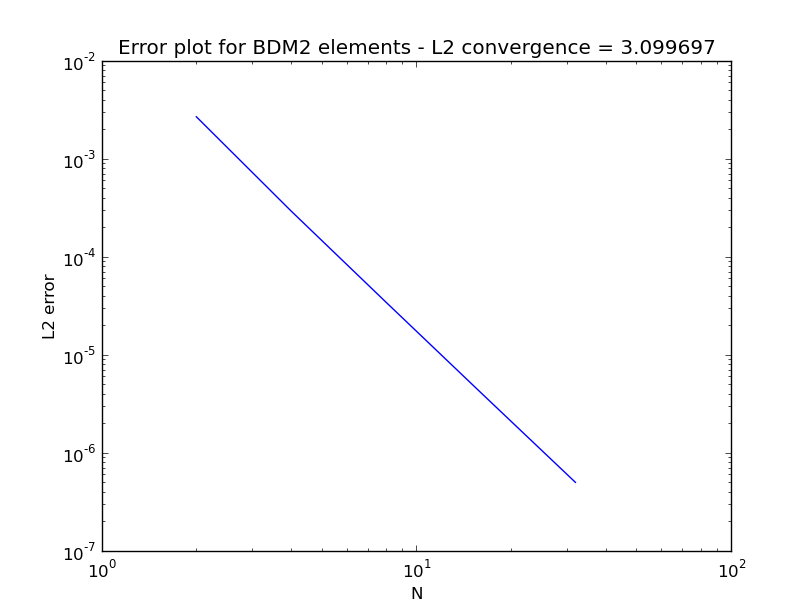
\includegraphics[width=10cm]{Plots/BDML2}
\end{figure}

\begin{figure}[h!]
\centering
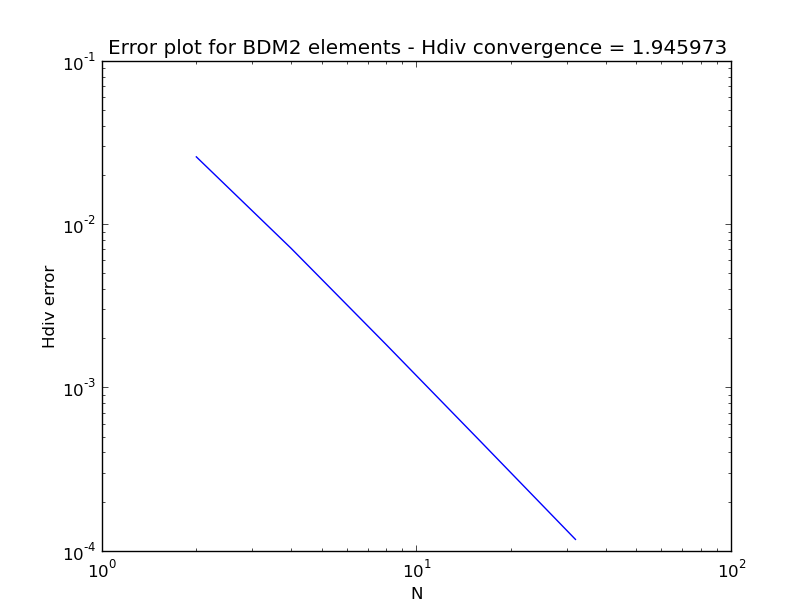
\includegraphics[width=10cm]{Plots/BDMHdiv}
\end{figure}

\begin{figure}[h!]
\centering
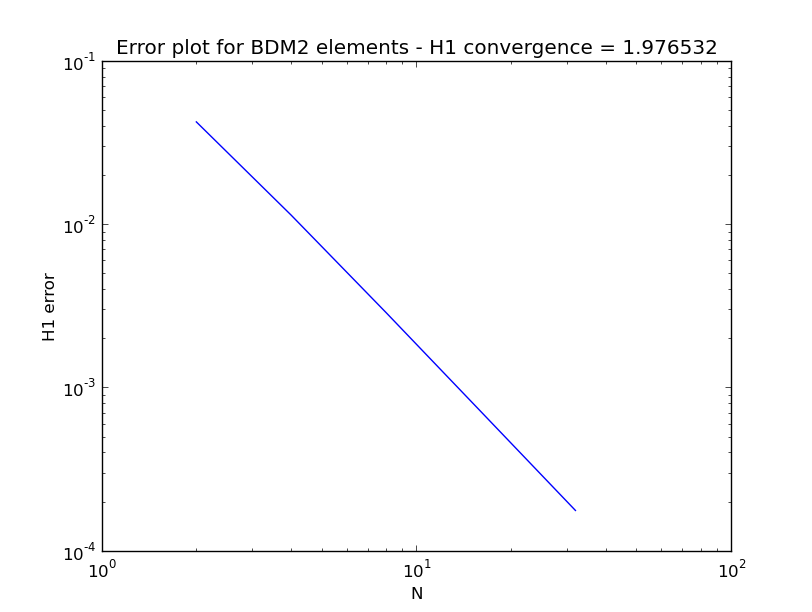
\includegraphics[width=10cm]{Plots/BDMH1}
\end{figure}

\begin{figure}[h!]
\centering
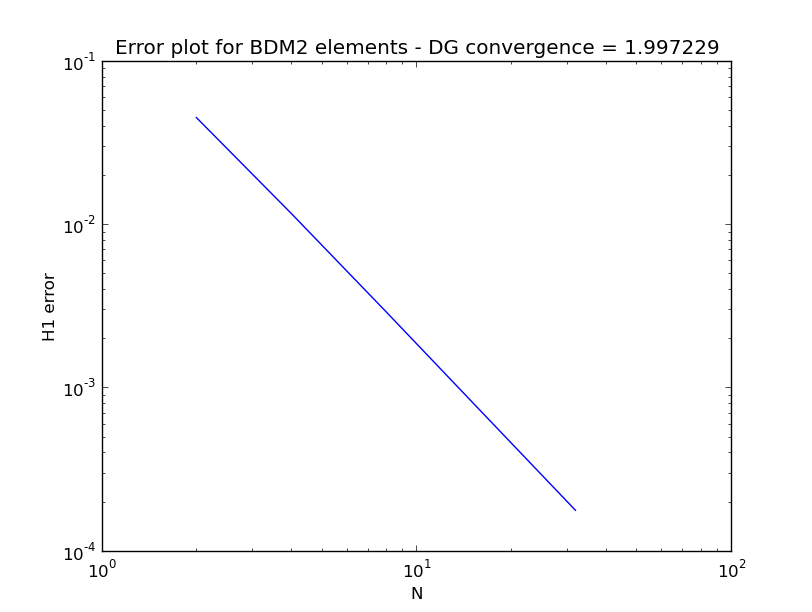
\includegraphics[width=10cm]{Plots/BDMDG}
\end{figure}


\newpage

\section*{CG vector Laplacian}

\begin{figure}[h!]
\centering
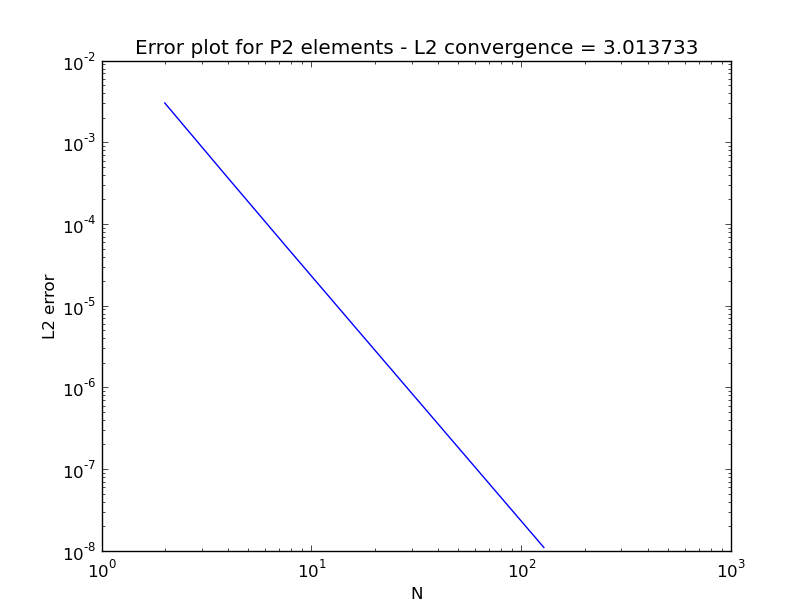
\includegraphics[width=10cm]{Plots/P2L2}
\end{figure}

\section*{Bilinear form}

Here is the new bilinear form for the Laplacian. We took care of the jump conditions on the between the triangles on the interior of the mesh but did not enforce anything on the boundaries. This is just for the DG scalar Laplacian but I was simple to extend this to the vector Laplacian.

\begin{python}
a = dot(grad(v), grad(u))*dx \
   - dot(avg(grad(v)), jump(u, n))*dS \
   - dot(jump(v, n), avg(grad(u)))*dS \
   + alpha/h_avg*dot(jump(v, n), jump(u, n))*dS \
   - dot(v*n, grad(u))*ds \
   - dot(grad(v), u*n)*ds \
   + gamma/h*v*u*ds
\end{python}

\end{document}
